\documentclass[11pt,a4paper]{ctexart}
\usepackage{tcolorbox,listings,hlist,enumerate,ulem,ifthen,ctex}
\usepackage[left=1cm,right=1cm,top=1.5cm,bottom=1.5cm]{geometry}
\usepackage{amscd,amssymb,amsfonts,amsbsy,amsmath,verbatim,color, mathrsfs,yhmath,tkz-euclide,chemfig,siunitx,circuitikz}
\usepackage[version=4]{mhchem}
\usepackage{asymptote}\usepackage{framed}
\usepackage{lastpage}
\usepackage{geometry} %调整页面边框
\geometry{a4paper,scale=0.8}%调整到80%
\usepackage{graphicx}
\usepackage{tikz}
\usepackage{multirow}%纵向合并表格
\usetikzlibrary{shapes.geometric,through,decorations.pathmorphing,arrows.meta,quotes,mindmap,shapes.symbols,shapes.arrows,automata,angles,3d,trees,shadows,automata,arrows,shapes.callouts,patterns,through,hobby}
\usetikzlibrary{intersections}%应用此 library 找到两条曲线的交点
\usetikzlibrary{calc} % 引入计算支持
\usepgflibrary{fpu}%调用 fpu 程序库,在计算线段与曲线、曲线与曲线的交点时使用这个库。
\newcommand{\RNum}[1]{\uppercase\expandafter{\romannumeral #1\relax}}%输入罗马数字
\usepackage{pgfplots}
\pgfplotsset{compat=1.17}
\usetikzlibrary{arrows}
\pagestyle{empty}
\usepackage{mathrsfs}
\usepackage{diagbox}%制作带斜线表头的宏包
\usepackage{pifont}%输入带圈数字
\usepackage{verbatim}%区间注释宏包
\usepackage{setspace}
\usepackage{fancyhdr}
\usepackage{tasks}
\settasks{label=\Alph*.,
	label-offset={0.5em},
	label-align=left,
	column-sep={2pt},
	item-indent={1.3em},before-skip={-0.7em},after-skip={-0.7em}}
\usepackage{ifthen}
\usepackage{array}

%---------- 选择题和填空题设置  --------------
  %选择题的4个选项,使用一个命令根据选项内容长度自动排版
\newlength{\lab}
\newlength{\lb}
\newlength{\lc}
\newlength{\ld}
\newlength{\lhalf}
\newlength{\lquarter}
\newlength{\lmax}
\newcommand{\xx}[4]{%%%%%%%%%
	\settowidth{\lab}{A.~#1~~~}
	\settowidth{\lb}{B.~#2~~~}
	\settowidth{\lc}{C.~#3~~~}
	\settowidth{\ld}{D.~#4~~~}
	\ifthenelse{\lengthtest{\lab > \lb}}  {\setlength{\lmax}{\lab}}  {\setlength{\lmax}{\lb}}
	\ifthenelse{\lengthtest{\lmax < \lc}}  {\setlength{\lmax}{\lc}}  {}
	\ifthenelse{\lengthtest{\lmax < \ld}}  {\setlength{\lmax}{\ld}}  {}
	\setlength{\lhalf}{0.5\linewidth}
	\setlength{\lquarter}{0.25\linewidth}
	\ifthenelse{\lengthtest{\lmax > \lhalf}}
	{%
		\begin{hlist}[pre skip=0pt,item skip=0pt,,item offset={1.5em}, label=\Alpha {hlisti}.,pre label={}]1
			\hitem #1
			\hitem #2
			\hitem #3
			\hitem #4
		\end{hlist}
	}  %%%
	{%%
		\ifthenelse{\lengthtest{\lmax > \lquarter}} % 
		{%
			\begin{hlist}[pre skip=0pt,item skip=0pt,item offset={1.5em}, label=\Alpha {hlisti}.,pre label={}]2
				\hitem #1
				\hitem #2
				\hitem #3
				\hitem #4
			\end{hlist}
		}
		{%
			\begin{hlist}[\parskip=0pt,pre skip=0pt,item skip=0pt,item offset={1.5em}, label=\Alpha {hlisti}.,pre label={}]4
				\hitem #1
				\hitem #2
				\hitem #3
				\hitem #4
			\end{hlist}
}}}

\newcommand{\tk}[2][2]{\uline{\makebox[#1cm][c]{%
				\ifanswer
				\textcolor{red}{#2}%
				\else
				\phantom{#2}%
				\fi}}}%填空答案
\newcommand{\kh}[1]{\hfill(\  {{%
			\ifanswer
			{\makebox[0.4cm][c]{\textcolor{red}{#1}}}%
			\else
			\phantom{\makebox[0.4cm][c]{#1} }%
			\fi}\  )}}%选择答案
	
\newif\ifanswer
\newcommand{\answer}[1]{\ifthenelse{\isodd{#1}}{\answertrue}{}}
\newcommand{\ty}[2]{\textcolor{blue}{\  {{%
				\ifty
				{%
				#1}%
				\else
				%\vspace*{8cm}%这里是空出的答题区域。也可以在exam-2022.tex中的题目下方插入合适的空白区域大小
				\fi}\  }}}%简答题答案/答案解析				
\newif\ifty
\newcommand{\tiyuan}[1]{\ifthenelse{\isodd{#1}}{\tytrue}{}}

\newcommand{\who}[1]{{{ %
			\ifwho
			{\hfill(\ \makebox[2.0cm][c]{\textcolor{blue}{#1}}\  )}%
			\else
			\phantom{\makebox[2.0cm][c]{#1} }%
			\fi}}}%(供题人:xxx)			
\newif\ifwho
\newcommand{\zuozhe}[1]{\ifthenelse{\isodd{#1}}{\whotrue}{}}
 \answer{1}%%1显示填空选择答案;0不显示
 \tiyuan{1}%%1显示简答题答案和解析文字;0不显示
 \zuozhe{1}%%1显示供题人;0不显示
\linespread{1.4}
%以下的这些包基本在setting文件里都有了,这里还是列出来不亏,请勿随意删除。请阅读一下settings文件,里面会发现很多在本说明中看不见的功能,篇幅限制无法一一注明。
\usepackage{ulem} %这个package是用来画删除线的
\usepackage{amssymb}
\usepackage{titlesec}%titlesec宏包调整section与正文间距
\usepackage{zref-user,zref-lastpage}%使用zref宏包,引用数字标签值和LastPage标签,感谢qingkuan大神指导
%\usepackage{times} %use the Times New Roman fonts
\usepackage{bigstrut}
\usepackage{enumerate}
\usepackage{amsmath,bm,amsthm,mathrsfs}
\everymath{\displaystyle}
\newcommand\dif{\mathop{}\!\mathrm{d}}
\def\d{\,\mathrm{d}}
\usepackage{tikz}%可以用于一些绘图
\usepackage{fancybox}
\usepackage{rotating}
\usepackage{tabularx}
\usepackage{wasysym}
\usepackage{color}

%%%%%%%%%%%%%%%%%%%%%%%%%%%%%%%%%%%%%%%
%增加新的一页,与自然形成的新一页相比,带一个题头。不需要题头就不用了
%%%%%%%%%%%
\def\d{\;\mathrm{d}}
\newcommand{\addpage}{
	\newpage
	 \begin{center}
    	\begin{Large}
    		\begin{center}
    			\textbf{仲英学业辅导中心 2021~-~2022 学年第一学期 期中考试模拟试题}
    			
    			{\zihao{5}  ~~仲英学业辅导中心~·~监制\hfill《线性代数与解析几何》期中模拟试题\hfill 第\;\thepage\;页~~ ~共 \pageref{LastPage}~页\hfill~~~
		  
		............................................装........................................订.......................................线............................................... \\[1mm]
	}


    		\end{center}
    	\end{Large}
    \end{center}\vspace{-5mm}}


\pagestyle{fancy} %页码显示
\renewcommand\headrulewidth{0pt}%隐藏页眉横线
\setlength\headheight{15pt}
  %  \cfoot{理科数学试卷\quad 第  \thepage 页(共 \pageref{LastPage}页)}
    \newcommand{\cndash}{\rule{0.2em}{0pt}\rule[0.35em]{1.6em}{0.05em}\rule{0.2em}{0pt}}%中文破折号
    \newcommand{\dotsbrack}{\dotfill (\qquad).}%选择题括号
   \newcommand{\blank}{\underline{\hspace{70pt}}}%填空题横线
 %%%%%%%%%%%%%%%%%%%%%%%%%%%%%%
 %%%%%%%%%%%%%%%%%%%%%%%%%%%%%%
\begin{document}
    \begin{center}
    	\begin{Large}
    		\begin{center}
    			\textbf{2021年高等数学I(上)期末试题}\\
    			% \textbf{《高等数学》}\\
    			% {\normalsize 仲英学业辅导中心 · 监制}\\
% {\zihao{5} 

		  
% 		............................................装........................................订.......................................线............................................... \\[1mm]
% 	}


    		\end{center}
    	\end{Large}
    \end{center}\vspace{-5mm}




\begin{framed}

    \begin{large}	
    \vspace{4mm} \noindent \textbf{一、选择题(共~5~题,每题~3~分)}
	\end{large}
    \begin{enumerate}

		\item  若\(\forall\; x \in \mathbb{R}\),总有\(\varphi(x) \leq f(x) \leq g(x)\),且\(\displaystyle \lim _{x \to \infty} (g(x) - \varphi(x)) = 0\),则以下关于\(\displaystyle \lim _{x \to \infty}f(x)\)的论述正确的是\kh{}
		\xx{存在且为\(0\)}{存在但不一定为\(0\)}{一定不存在}{不一定存在}

		\item 使不等式\(\displaystyle \int_1^x \frac{\sin t}{t}\d t > \ln x\)	成立的\(x\)的范围是\kh{}
		\xx{\(\displaystyle \left( 1, \frac{\pi}{2}\right)\)}{\(\displaystyle \left(  \frac{\pi}{2},\pi\right)\)}{\((0, 1)\)}{\((\pi, +\infty)\)}
		
		\item 设\(f(x)\),\(g(x)\)	是恒大于零的可导函数,且\(f'(x)g(x) - f(x)g'(x) < 0\),则当\(a < x < b\)时,有\kh{}
		\xx{\(f(x) g(b) > f(b)g(x)\quad\)}{\(f(x)g(a) > f(a)g(x)\)}{\(f(x)g(x) > f(b)g(b)\)}{\(f(x)g(x) > f(a)g(a)\)}

		\item 设函数\(f(x) \in C[-1, 1]\),则\(x = 0\)是函数\(g(x) = \displaystyle\frac{\displaystyle \int_0^xf(x) \d x}{x}\)的\kh{}\xx{第一类跳跃间断点\qquad }{第一类可去间断点}{第二类无穷间断点}{连续点}

		\item 如下图所示,曲线段的方程为\(y = f(x)\)	,且函数\(f(x)\)	在区间\([0, a]\)上有连续的导数,则定积分\(\int_0^a xf'(x)\d x \)表示的是 \kh{}
		
		\begin{center}
			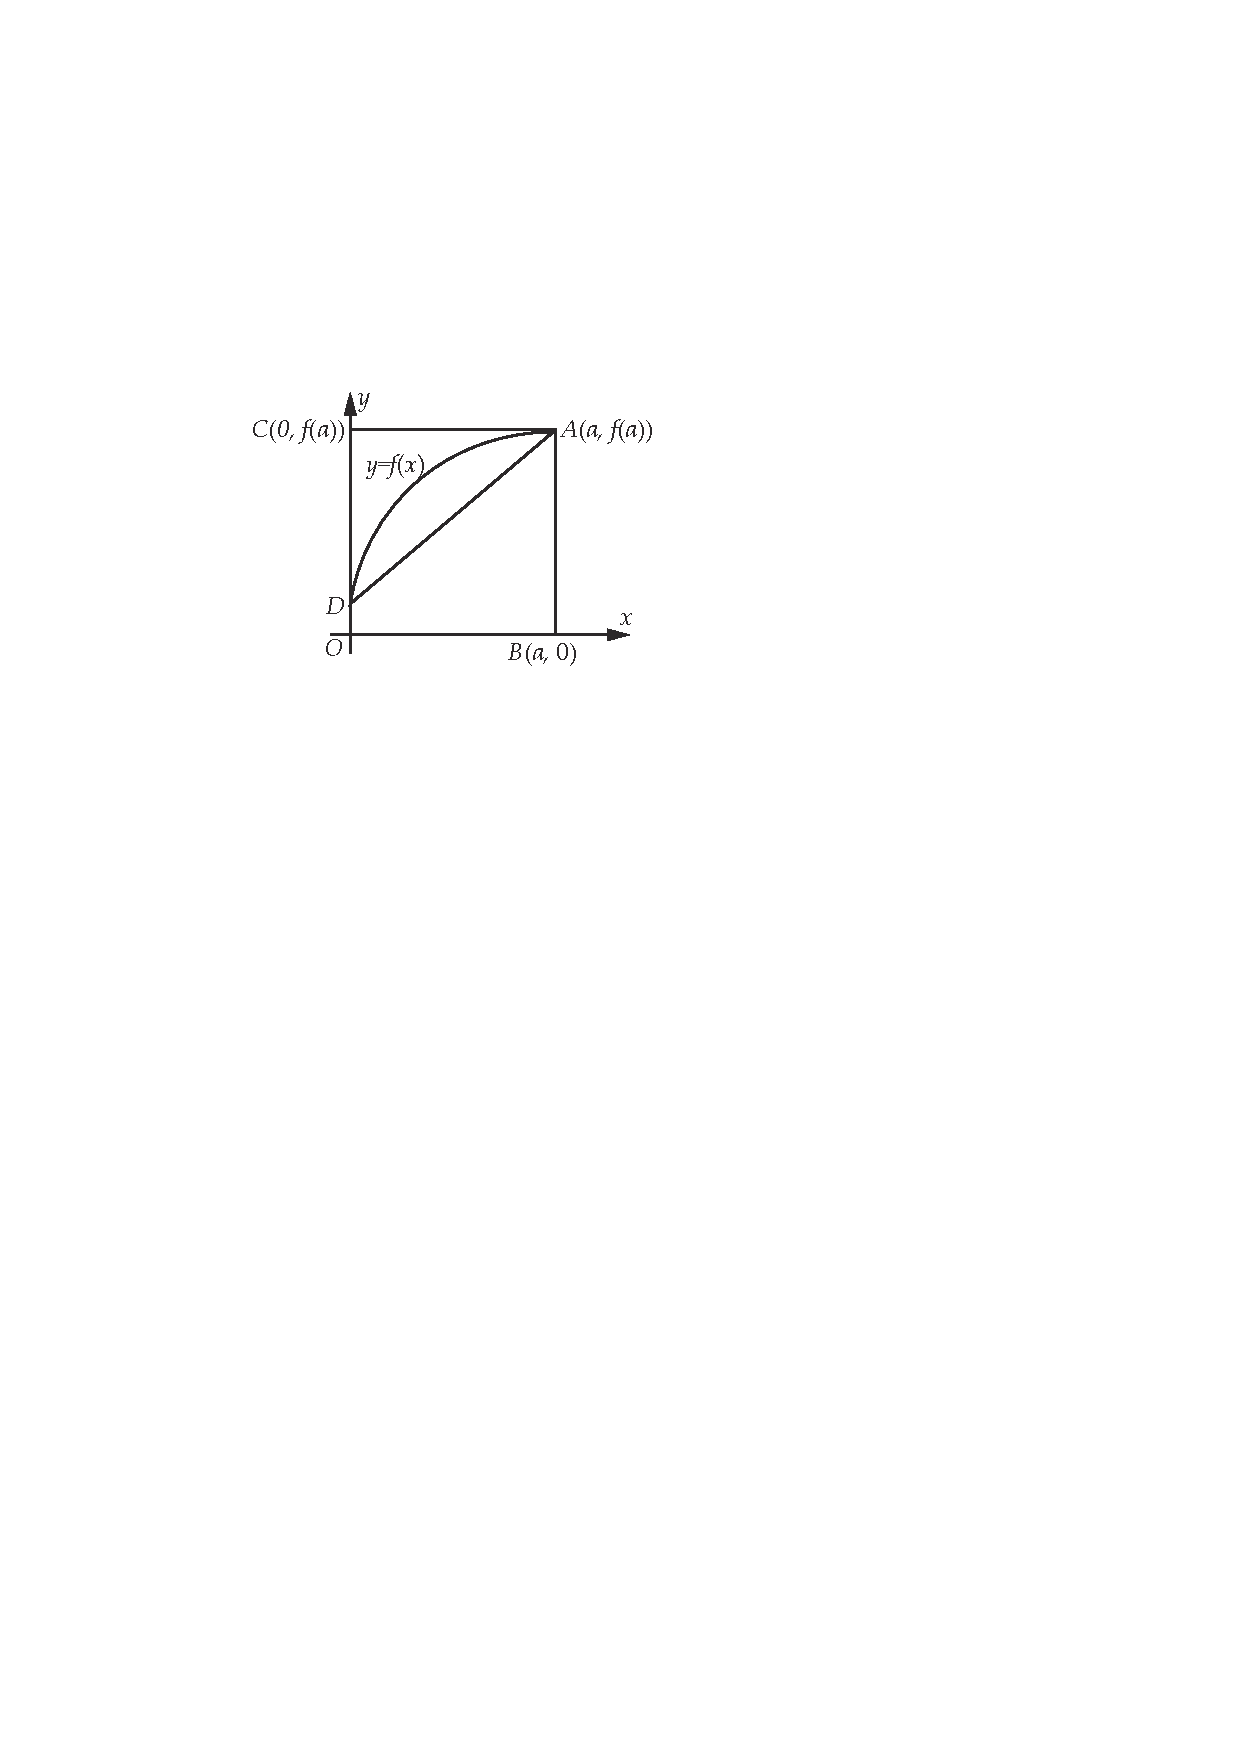
\includegraphics[scale = 0.7]{fig/figure1.pdf}
		\end{center}

		 \xx{曲边梯形\(ABOD\)的面积}{梯形\(ABOD\)的面积}{曲边三角形\(ACD\)的面积}{三角形\(ACD\)的面积}

		
		

		
	\end{enumerate}
	\begin{large}
			\noindent\textbf{二、填空题(共~5~题,每题~3~分)}
	\end{large}        
	\begin{enumerate}
		% \setcounter{enumi}{5}%从5开始计数,用于更改题号

		\item 设\(f(x + 1) = \displaystyle \lim_{n \to \infty} \left(\frac{n + x}{n - 2}\right)^x\),则\(f(x) = \)\tk{}.

		\item 设\(f(x) = \displaystyle \lim _{t \to+\infty} \frac{x^2e^{t(x - 2) }+ ax - 1}{e^{t(x - 2)} + 1}\)	在\((-\infty, +\infty)\)内连续,则常数\(a = \)\tk{}.
		
		\item \(\displaystyle \int_0^\pi (f(x) + f''(x)) \sin x \d x = 5,\; f(\pi) = 2\),则\(f(0) = \)\tk{}.
		
		\item 设\(f(x) = \displaystyle \int_0^{x^2} (e^{-t^2} + 6)\d t\),则\(\displaystyle \lim_{\alpha \to 0}\frac{f(x + \alpha) - f(x - \alpha)}{\alpha} = \)\tk{}.

		\item \(\displaystyle \lim_{n \to +\infty} \frac{1^p + 2^p + \cdots + n^p}{n^{p + 1}} = \)\tk{}.其中常数\(p > 0\).
 
	\end{enumerate}    
% \end{framed}
% %%%%%%%%%%%%%%%%%%%%%%%
%   \addpage  \begin{framed}

	\begin{large}
		\noindent\textbf{三、计算题(共~7~题,每题~6~分)}
	 \end{large}

	 \begin{enumerate}
		\item 计算极限\(\displaystyle \lim_{x \to 0} \frac{e^x\sin x - x - x^2}{(e^x - 1) \sin ^2x}\).\[\] \[\]\[\]\[\]\[\]\[\]\[\]\[\]\[\]\[\]
		\item 设\(f(x) = \left\{\begin{aligned}
			&\sin x + 2ae^x, & & x < 0\\
			&9\arctan x + 2b(x - 1)^3,& & x \geq 0
		\end{aligned}\right.\),试确定常数\(a, b\)的值,使得函数\(f(x)\)在其定义域上可导.\[\] \[\]\[\]\[\]\[\]\[\]\[\]\[\]\[\]\[\]
		\item 求函数\(f(x ) = x - 2 \arctan x	\)的单调区间、极值和其对应曲线的凹凸区间以及渐近线,并画出此函数的简单示意图.\[\] \[\]\[\]\[\]\[\]\[\]\[\]\[\]\[\]\[\]
		\item 计算定积分\(\displaystyle \int_0^3 \arcsin \sqrt[]{\frac{x}{x + 1}}\d x\).\[\] \[\]\[\]\[\]\[\]\[\]\[\]\[\]\[\]\[\]
		\item 计算不定积分\(\displaystyle \int \frac{x^3}{\sqrt[]{1 + x^2}}\d x.\)\[\] \[\]\[\]\[\]\[\]\[\]\[\]\[\]\[\]\[\]
		\item 设\(\displaystyle f(x) = \frac{(x+1)^2 (x - 1)}{x^3 (x - 2)}\),计算\(\displaystyle I = \int_{-1}^3 \frac{f'(x)}{1 + f^2 (x) } \d x.\) \[\] \[\]\[\]\[\]\[\]\[\]\[\]\[\]\[\]\[\]
		\item 假设由抛物线\(y = x^2,\; y = 4x^2\)以及直线\(y = H\;(H > 0)\)围成的平面图形绕\(y\)轴旋转一周形成的旋转抛物面型容器内盛满水,若将水全部抽出,需要作多少功?\[\] \[\]\[\]\[\]\[\]\[\]\[\]\[\]\[\]\[\]
	 \end{enumerate}


	\begin{large}
       \noindent\textbf{四、(8分)}
	\end{large}
	求微分方程\((2x - 1)^2 y'' + 4(2x - 1)y' - 8y = 4x - 3\)的通解.\[\] \[\]\[\]\[\]\[\]\[\]\[\]\[\]\[\]\[\]

	\begin{large}
		\noindent\textbf{五、(8分)}
	\end{large}
	求微分方程组\(\displaystyle \frac{\d\boldsymbol{x}}{\d t} = \begin{pmatrix}
		2 & 1 & 0 \\ 0 & 2 & 0 \\ 0 & 1 & 3 \\
	\end{pmatrix}\boldsymbol{x} + \begin{pmatrix}
		t\\1\\0
	\end{pmatrix}\)的通解.\[\] \[\]\[\]\[\]\[\]\[\]\[\]\[\]\[\]\[\]

	\begin{large}
		\noindent\textbf{六、(6分)}
	\end{large}
	设函数	\(f(x)\)在\([0, 2 \pi]\)上连续,在\((0, 2\pi)\)内可导,且\(f(0) = 1,\; f(\pi) = 3,\; f(2\pi)  = 2\).试证明在\((0, 2\pi)\)内至少存在一点\(\xi\),使得\(f'(\xi) + f(\xi) \cos \xi = 0.\)\[\] \[\]\[\]\[\]\[\]\[\]\[\]\[\]\[\]\[\]

	\begin{large}
		\noindent\textbf{七、(6分)}
	\end{large}
	设函数\(f(x), g(x)\)是\([-a, a]\)上的连续函数,\(g(x)\)	是偶函数,\(f(-x) + f(x) = A\)(\(A\)是常数).\begin{enumerate}[(1)]
		\item 证明:\(\displaystyle \int_{-a}^a f(x) g(x) \d x = A \int_0^a g(x) \d x\);
		\item 计算定积分\(\displaystyle \int_{-\frac{\pi}{2}}^{\frac{\pi}{2}} \cos^4x \arctan e^x \d x.\)
	\end{enumerate}
	\[\] \[\]\[\]\[\]\[\]\[\]	\[\] \[\]\[\]\[\]\[\]\[\]

	
	
    

    
    \end{framed}
  
\end{document}